%\documentclass[12pt, twoside]{article}
%\documentclass[12pt]{article}%REMOVE AFTER
\documentclass[sn-mathphys-num]{sn-jnl}
\usepackage{a4wide}%REMOVE AFTER

%\usepackage{jmlda}
\usepackage[title]{appendix}%
\usepackage[utf8]{inputenc}
\usepackage[english]{babel}
\usepackage[T2A]{fontenc}
\usepackage{lineno}
\usepackage{amssymb,amsfonts,amsmath,mathtext}
\usepackage{amsthm}
\usepackage{array}
%\usepackage{theorem}
\usepackage[all]{xy}
\usepackage{array}
\usepackage{multicol}
\usepackage{hhline}
\usepackage{graphicx}
\usepackage{float}
\usepackage{subcaption}
\usepackage{wrapfig}%Обтекание фигур (таблиц, картинок и прочего)
\usepackage{multirow}
\usepackage{pgfplots}
\pgfplotsset{compat=1.9}
\usepackage{graphicx}%
\usepackage{mathrsfs}%
\usepackage[title]{appendix}%
\usepackage{xcolor}%
\usepackage{textcomp}%
\usepackage{manyfoot}%
%\usepackage{booktabs}%
\usepackage{algorithm}%
\usepackage{algorithmicx}%
\usepackage{algpseudocode}%
\usepackage{listings}%
\renewcommand{\thesubfigure}{\textit{\alph{subfigure}}}
\graphicspath{{figures/}}   
\newcommand{\hdir}{.}

\theoremstyle{thmstylethree}
\newtheorem{definition}{Defenition}
\theoremstyle{thmstyletwo}
\newtheorem{remark}{Remark}

\theoremstyle{thmstyleone}
\newtheorem{theorem}{Theorem}
\newtheorem{lemma}{Lemma}

\raggedbottom
\begin{document}
%\English

\title
	[Classification of trajectories of dynamic systems using
physically-informed neural networks] % short title for page headings, not necessary if a full title fits the headings
    {Classification of trajectories of dynamic systems using
physically-informed neural networks} % full title
\author*[1]{\fnm{V.} \sur{Strizhov}}\email{iauthor@gmail.com}
\author*[2]{\fnm{A.} \sur{Terentyev}}\email{iauthor@gmail.com}

\affil*[1]{\orgdiv{Department}, \orgname{Organization}, \orgaddress{\street{Street}, \city{City}, \postcode{100190}, \state{State}, \country{Country}}}

\affil[2]{\orgdiv{Department}, \orgname{Organization}, \orgaddress{\street{Street}, \city{City}, \postcode{10587}, \state{State}, \country{Country}}}

\abstract
{The paper proposes a method for multivariate time series classification using information about their physical nature. The paper proposes a classification model for multidimensional trajectories of physical systems. In comparison to models that use assumptions about statistical properties of trajectories only, but do not use  prior information, the presented model includes information about the physical nature of the system. It makes the classification stable to random non-physical changes in trajectories. To account for these changes we train the model on augmented samples. We propose to classify not the trajectories themselves, but the dynamical systems given by the Lagrangians corresponding to these trajectories. The Lagrangian is reconstructed using physics-informed Lagrangian neural networks. We introduce a norm in the space of Lagrangians and use it in metric classification. 

\textbf{Keywords}: \emph{physical system; Lagrangian; Lagrangian neural network; compactness hypothesis}}

%these fields are filled in by the journal editors
%\doi{10.21469/22233792}
%\receivedEng{January 01, 2017}

\maketitle
%\linenumbers

\section{Introduction}

The physics-informed neural networks (PINNs) combine the advantages of statistical and mathematical models. The first ones fit the measured data while the second ones take a physical description of the modeled system into account. The PINNs model conservation laws using data as the basis for predictions. Its architecture is analyzed in~\cite{PINNreview}. PINNs model principles of Hamiltonian~\cite{HNN}, Lagrangian dynamics~\cite{article}, including Hamiltonian mechanics with infinite-dimensional measurement space~\cite{quantumHNN} from
quantum physics. The Lagrangian networks (LNN) also adapt to model microsystems using graph networks~\cite{LGNN}. The modifications of LNN model complex macro-systems such as fluids with the multi-particle approximation~\cite{fluid-LNN}. Also, PINNs allows dimension reduction using special operator~\cite{HNNreduce}. PINNs and LNNs also reconstruct sound~\cite{PINNsoundwave} taking into account wave equations. 

The paper \cite{HNNadapt} introduces Hamiltonian neural networks to adapt a nonlinear variation of a parametrized system and determine the parameter of nonlinearity. This parameter is responsible for the chaotic nature of the system, acting as a measure of chaos and separating the chaotic system from the original system. The disadvantage of this classification is that one needs to know in advance the law by which these systems are separated. According to \cite{HNNrobustclass} Neural Ordinary Differential Equations (NODE) could be unstable due to changes in the initial data, and the error grows exponentially in time. The architecture of CH-NODE reduces these shortcomings but in general, the classification problem for systems with Lagrangian dynamic remains unexplored.

Mostly convolutional neural networks are used for multivariate classifications, assuming that there are statistical relationships between the closest points of the time series~\cite{TCSreview}. These methods perform well in many tasks where these relationships are predominant. But for physical systems such methods are not suitable, and it is proposed to use knowledge about physical connections of systems, for the selected Lagrangian neural networks this knowledge is the law of conservation of energy.	

This paper solves the problem of dynamic system trajectory classification. It proposes to use Lagrangian neural networks (LNN) for low-dimensional trajectories. Each trajectory refers to the Lagrangian of the system parameterized by the LNN. The issue of mapping the Lagrangian of the system along the trajectory is analyzed in~\cite{article}.

The dynamical system's state and its trajectory are constructed with multivariate time serties~\cite{TCSreview}. Deep learning methods, developed for the univariate time series, like AlexNet, ResNet, InceptionTime, TapNet~\cite{TCSreview}\cite{MTCSreview} need architecture updates for the data acquired from several sensors~\cite{MTCSindustrial} including three-axis accelerometer and gyroscope~\cite{MTCSactivity} and updates for the knowledge about the physical description of the dynamic system. The state-of-art approach in this field is using randomized kernels ROCKET, however it doesn't outperform others on all datasets~\cite{TCSreview}\cite{ROCKET}.

The Lagrangian network reconstructs system trajectories where the conservation of energy and the Euler-Lagrange equations hold. The LNN  uses an independent set of coordinates to specify the state of the system. In the Lagrangian formalism, the dynamic system is defined by the Lagrangian function.  The generalized coordinates in Lagrangian mechanics specify the state of the system. The minimum number of independent variables (generalized coordinates) necessary for a description of the state of the mechanical system is chosen. The Lagrangian of the system is a continuous differentiable and square-integrable function. Its Euler-Lagrange equation has a unique solution. 
The dynamic system is described by the Euler-Lagrange equation,
\begin{equation}
\frac{\partial L}{\mathbf{q}}-\frac{d}{dt}\frac{\partial L}{\partial\dot{\mathbf{q}}}=Q_x=0.
      \label{eq:euler_larange}
\end{equation}
For its unique solution, the necessary and sufficient condition is 
\begin{equation}
    \det \left \| \frac{\partial^{2} L}{\partial \dot{q}_{j}\partial \dot{q}_{k}} \right \|_{j,k=1}^{n} \neq 0.
\end{equation}
\begin{figure}
\centering
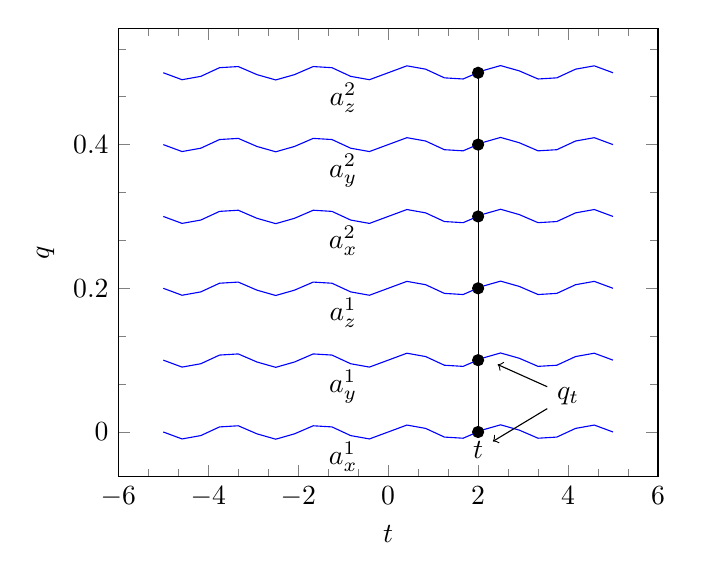
\begin{tikzpicture}
\begin{axis}[
	xlabel = {$t$},
	ylabel = {$q$},
	minor tick num = 2
]
\addplot[draw = blue, mark options=black] {sin(x  * 180) * 0.01 + 1/10 * 0}
node[pos=0.4,below] {$a^1_x$};
\addplot[draw = blue, mark options=black] {sin(x  * 180) * 0.01 + 1/10 * 1}
node[pos=0.4,below] {$a^1_y$};
\addplot[draw = blue, mark options=black] {sin(x  * 180) * 0.01 + 1/10 * 2}
node[pos=0.4,below] {$a^1_z$};
\addplot[draw = blue, mark options=black] {sin(x  * 180) * 0.01 + 1/10 * 3}
node[pos=0.4,below] {$a^2_x$};
\addplot[draw = blue, mark options=black] {sin(x  * 180) * 0.01 + 1/10 * 4}
node[pos=0.4,below] {$a^2_y$};
\addplot[draw = blue, mark options=black] {sin(x  * 180) * 0.01 + 1/10 * 5}
node[pos=0.4,below] {$a^2_z$};
\addplot [draw = black, mark=*, mark options=black] coordinates{(2,0) (2, 0.1) (2, 0.2) (2, 0.3) (2, 0.4) (2, 0.5)}
node[pos=0,below] (q1){$t$}
node[pos=0.2, right] (q2){};
\node (qt) at (axis cs:4, 0.05){$q_t$};
\draw[->](qt)--(q1);
\draw[->](qt)--(q2);
\end{axis}
\end{tikzpicture}
\end{figure}
The equivalent physical definition of the Lagrangian is the difference between the kinetic~$T$ and potential~$V$ energy,
\begin{equation}
L\left(\mathbf{q},\dot{\mathbf{q}}\right) = T\left(\mathbf{q},\dot{\mathbf{q}}\right)- V\left(\mathbf{q},\dot{\mathbf{q}}\right), 
\label{eq:L=T-V}
\end{equation}
where~$\mathbf{q}_t$ are the generalized coordinates of the system, $\dot{\mathbf{q}}_t$~are the generalized accelerations of the system, $L$~is the Lagrangian of the system.

For Lagrangians of different motions of a physical system, we assume the compactness hypothesis: the Lagrangians which correspond to different motions lie in different compact and separable subsets. We label these subsets as the classes in the space of trajectory models. We assume the parameters of these models are also separable for different classes. The computational experiment uses the PAMAP2 dataset~\cite{misc_pamap2_physical_activity_monitoring_231}. The dataset contains trajectories of human movements during common daily activities like cooking, jogging, and shopping.

The
dataset contains recordings from three sets of gyroscopes and accelerometers: attached to the
wrist of the dominant arm, attached to the chest, attached to the elbow of the predominant hand. Number of subjects is 9. Number of activity types(classes) is 24, each activity lasted 2-4 minutes ~\cite{misc_pamap2_physical_activity_monitoring_231}, sampling frequency 100 Hz. This dataset provides data from different part of dynamic system. Which provides an opportunity to consider the performance of the algorithm on a complex dynamic system. Since that, we consider general coordinates for the system consist of coordinates of all sensors that are used in experiments as one vector.

\section{Formulation of the regression problem for a time series and
Lagrangian neural networks}

Assume that the Lagrangian~$L$  of the dynamical system corresponds to some specific trajectory. The Lagrangian defines a dynamical system for which the trajectory is constructed: substituting~$L$ into the
Euler-Lagrange equation~\eqref{eq:euler_larange} yields a function relating the velocity and coordinates of the point to its acceleration. By solving the ODE system obtained by substituting~$L$ into~\eqref{eq:euler_larange}, with initial conditions, the initial point of the trajectory, the trajectory is fully recovered.  We identify each trajectory by some function~$L$ from the space with norm $L_2$ and identify the trajectory and the dynamical system, given by the function~$L$, which we further feed to the input of the classifier. The problem of recovery~$L$ we formulate as the regression problem.

Denote by~$X$ the trajectory of dimension~$r$ and length~$T$ 
\begin{equation}
X = [\mathbf{X}_1,\dots, \mathbf{X}_T] \quad \text{where} \quad \mathbf{x}_i = (\mathbf{q}_i, \dot{\mathbf{q}}_i), \quad  \text{and}\quad \dot{\mathbf{q}}_i \in \mathbb{R}^r
\label{definition:trajectory}
\end{equation}
is the velocity at the $i$-th time-tick, and $\mathbf{q}_i \in \mathbb{R}^r$  is the coordinate at the $i$-th time-tick.

There given a sample set 
\begin{equation}
D = \{(\mathbf{x}_i, \mathbf{y}_i)\}_{i=1}^N,
\label{eq:dataset}
\end{equation}
where $X$ are trajectories of dimension $r$ and length $T$, $\mathbf{y}_i = \ddot{\mathbf{q}}_i \in \mathbb{R}^r$ is the acceleration at the $i$-th time-tick. One has to find a function that predict acceleration for particular point, using previous data $D$
\begin{equation}
\hat{\mathbf{y}}  = \mathbf{f}(\mathbf{x} | D),
\quad
\text{where}
\quad
\hat{Y} = \{\hat{\mathbf{y}}_i = \hat{\ddot{\mathbf{q}}}_i\}_{i=1}^N
\label{eq:model}
\end{equation}
is the predicted trajectory of the dynamic system. The function~$\mathbf{f}=\mathbf{f}(\mathbf{x} | \mathbf{w})$ with parameters~$\mathbf{w}$ is selected from the family  of Lagrangian neural networks.

The loss function of the predicted acceleration~$\hat{\mathbf{y}}_i$ given the points $\mathbf{X}_i = (\mathbf{q}_i, \dot{\mathbf{q}}_i)$ of the trajectory $X$ is 
\begin{equation}
 \mathcal{L}(\textbf{w}) = \mathcal{L}(\mathbf{w} | D) = \frac{1}{T}\sum_{i=1}^{T} \| \hat{\mathbf{y}}_i - \mathbf{y}_i \|_2^2.
\end{equation}
To fit the parameters of the neural network one hes to solve the optimization problem
\begin{equation} 
\label{eq:opt_task}
\textbf{w}_j^* = \arg\min_{\mathbf{w} \in \mathbb{W}} \bigl( \mathcal{L}(\textbf{w}) \bigr). 
\end{equation}

The algorithm of modeling the dynamic system with  Lagrangian is:
\begin{enumerate}
	\item Find analytical expressions for the kinetic~$T$ and the potential~$V$ energies.
	\item Get the Lagrangian~$L=T-V$ in~\eqref{eq:L=T-V}.
	\item Apply the Euler-Lagrange constraint~\eqref{eq:euler_larange}.
	\item Solve the resulting system of differential equations.
\end{enumerate}

Instead of parametrizing dynamic system by Neural network
\begin{equation}
\hat{\mathbf{y}}  = \mathbf{f}(\mathbf{x} | \mathbf{w}),
\quad
\text{where}
\quad
\mathbf{w} \text{~-- parameters of neural netowork,}
\label{eq:model}
\end{equation}

To add prior knowledge of the physics of the system we model the Lagrangian:
\begin{equation}
\hat{L}  = f(\mathbf{x} | \mathbf{w}),
\quad
\text{where}
\quad
\hat{L}\text{~--estimation of Lagrangian at point}~\mathbf{x}.
\end{equation}
The key idea is to fit the Lagrangian~$L$ by a neural network~$f$, one has to obtain the expression of the Euler-Lagrange constraint and back propagate the error through this constraint:
\begin{equation}
\ddot{\mathbf{q}} =\left(\nabla_{\dot{\mathbf{q}} \dot{\mathbf{q}}} L\right)^{-1}\left[\nabla_{\mathbf{q}} L-\left(\nabla_{\dot{\mathbf{q}}\mathbf{q}} L\right) \dot{\mathbf{q}}\right].
\label{eq:euler_larange_to_acc}
\end{equation}
The diagram of the proposed neural network is
%\begin{figure}
%\centerline{
\begin{equation}
    \xymatrix{
    \mathbf{x}_i = (\mathbf{q}_i, \dot{\mathbf{q}}_i) \ar@{->}[rrr]^-{\hat{L} \colon (\mathbf{x} | \mathbf{w}) \to L_\mathbf{x}} & & & L_\mathbf{x} \ar@{->}[r]^-{\nabla L} & \frac{d}{d t} \frac{\partial L}{\partial \dot{\mathbf{q}}} =\frac{\partial L}{\partial \mathbf{q}} \ar@{->}[rr]^-{{\ddot{\mathbf{q}}_i = g\left(\mathbf{q}_i, \dot{\mathbf{q}}_i\right)}} &  & \mathbf{y}_i = \ddot{\mathbf{q}}_i
    }.
%}
\label{fig: LNN}
\end{equation}
The neural network $\hat{L} \colon (\mathbf{x} | \mathbf{w}) \to L_\mathbf{x}$ from~\eqref{fig: LNN} is a fully-connected network with three layers with the SoftPlus activation function.  One has to estimate $\hat{L}$ of the Lagrangian~$L$, differentiate $\hat{L}$ and obtain~$\nabla_{\dot{\mathbf{q}}\dot{\mathbf{q}}}\hat{L}$, $\dot{\mathbf{q}}\hat{L}$, and~$\nabla_{\dot{\mathbf{q}}\mathbf{q}} \hat{L}$ at point $\mathbf{x}$. To obtain the acceleration~$\hat{\mathbf{y}}$, the values of the gradients are substituted into the Euler-Lagrange equation \eqref{eq:euler_larange} in the form \eqref{eq:euler_larange_to_acc}, from which one has to estimate~$\hat{\mathbf{y}}$. For the given coordinates~$(\mathbf{q}, \dot{\mathbf{q}})$ we have a model with prior knowledge of the energy conservation which obtains the dynamics~$(\dot{\mathbf{q}}, \ddot{\mathbf{q}})$. 

\section{Approximation of the norm in Lagrangian space}
We assume the Lagrangians of trajectories are compact. 
%This assumption is based on the fact that different muscle groups produce different human movements. And similar ones are based on similar ones. Therefore, different in nature movements will form different mechanical systems and vice versa. Hence the hypothesis naturally follows. It remains to test this hypothesis. For this purpose, it is necessary to clarify the terms mentioned in the first paragraph.
Denote by~$\mathbb{L}$ the functional Lagrangian space:
\[ 
\hat{L} =  \mathbf{x} \to L_x, \quad g \in \mathbb{L},
\] 
where~$\mathbf{x} \in \mathbb{R}^{2 \times r}$ is the vector of generalized coordinates and velocities, $L \in \mathbb{R}$ is the value of the Lagrangian of the dynamic system. The parametric family of functions~\eqref{eq:model} approximate the Lagrangian
\[
 \mathbb{L}_{\epsilon} = \{ \hat{L}^{(\epsilon)} \colon (\mathbf{x} | \mathbf{w}) \to \hat{L}(\mathbf{x}) \mid \mathbf{x} \in \mathbb{R}^{2 \times r}, \hat{L}(\mathbf{x})  \in \mathbb{R}\}, \quad \mathbb{L}_{\epsilon} \subset \mathbb{L},
\]
where $\mathbf{w}$ is the vector of parameters of the approximation model, $\epsilon$~is the approximation accuracy.

To construct the norm, obtain a system of equations  and calculate the accelerations. The Lagrangian formalism models the dynamic system with coordinates~$\mathbf{x}_t = (\mathbf{q}, \dot{\mathbf{q}})$. It starts in the state~$\mathbf{x}_0$ and ends in the state~$\mathbf{x}_1$. Define the action  
\[ %\begin{equation}
S=\int_{t_{0}}^{t_{1}} L d t.
\]% \end{equation}
The action defines a path from~$\mathbf{x}_0$ to~$\mathbf{x}_1$ with the coordinates~$\mathbf{x}_t$ in the time interval $t_0, t_1$. The path minimizes the action $S$. %, i.e. $\delta S = 0$. 
The solution is the Euler-Lagrange equation~\eqref{eq:euler_larange}. It defines the system dynamics. 
%\begin{equation}
%\frac{d}{d t} \frac{\partial L}{\partial \dot{\mathbf{q}}}=\frac{\partial L}{\partial \mathbf{q}}.
%\end{equation}
Obtain the acceleration of each component~$ \ddot{\mathbf{q}}$ from the chain rule. Write the time derivative through the coordinate derivatives:
\[
\left(\frac{\partial}{\partial \mathbf{q}} \frac{\partial L}{\partial \dot{\mathbf{q}}} \right) \frac{d q}{d t}+\left(\frac{\partial}{\partial \dot{\mathbf{q}}} \frac{\partial L}{\partial \dot{\mathbf{q}}} \right)  \frac{d \dot{\mathbf{q}}}{d t}
= \frac{\partial L}{\partial \mathbf{q}}.
\]
Rewrite the time derivatives for clarity
\[
\frac{\partial}{\partial \mathbf{q}} \frac{\partial L}{\partial \dot{\mathbf{q}}} \dot{\mathbf{q}}+\frac{\partial}{\partial \dot{\mathbf{q}}} \frac{\partial L}{\partial \dot{\mathbf{q}}} \ddot{\mathbf{q}} 
= \frac{\partial L}{\partial \mathbf{q}}.
\]
Move the summands so that only the unknowns ones remain on the left side:
\[
\frac{\partial}{\partial \dot{\mathbf{q}}} \frac{\partial L}{\partial \dot{\mathbf{q}}} \ddot{\mathbf{q}} 
= \frac{\partial L}{\partial \mathbf{q}}-\frac{\partial}{\partial \mathbf{q}} \frac{\partial L}{\partial \dot{\mathbf{q}}} \dot{\mathbf{q}}.
\]
Divide both parts to get  the unknown variable:
\[
\ddot{\mathbf{q}} 
= \left(\frac{\partial}{\partial \dot{\mathbf{q}}} \frac{\partial L}{\partial \dot{\mathbf{q}}}\right)^{-1}\left[\frac{\partial L}{\partial \mathbf{q}}-\frac{\partial}{\partial \mathbf{q}} \frac{\partial L}{\partial \dot{\mathbf{q}}} \dot{\mathbf{q}}\right].
\]
Rewrite the partial derivatives with nabla-notation:
\begin{equation}
\ddot{\mathbf{q}} 
= \left(\nabla_{\dot{\mathbf{q}} \dot{\mathbf{q}}} L\right)^{-1}\left[\nabla_{q} L-\left(\nabla_{\dot{\mathbf{q}}\mathbf{q}} L\right) \dot{\mathbf{q}}\right], \quad\text{where the Hessian}\quad
\mathbf{H} = \nabla_{\dot{\mathbf{q}}\dot{\mathbf{q}}} L = \frac{\partial^{2} L}{\partial \dot{\mathbf{q}} \partial \dot{\mathbf{q}}}.
\end{equation}

The condition $\det \mathbf{H} \neq 0$ at any point  must be held since we assume non-degenerate system of linear equations.
\begin{equation}
\label{eq:linear_equation_acc}
\mathbf{H}\ddot{\mathbf{q}} 
= \frac{\partial L}{\partial \mathbf{q}}-\frac{\partial}{\partial \mathbf{q}} \frac{\partial L}{\partial \dot{\mathbf{q}}} \dot{\mathbf{q}},
\end{equation}

\begin{lemma} \label{lemma1}
If the Lagrangians are set on a compact, then there exist non-negative numbers $a, b$ such that $\det \mathbf{H} \ge a$ and the eigenvalues of the matrix $\mathbf{H}$ are at least $b$.
\end{lemma}
\begin{proof}
Assume the opposite: $\mathbf{H}$~is a continuous function since its values are the second derivatives of~$L$, hence~$\det \mathbf{H}$ and its eigenvalues are also continuous and hence reach their minimum and maximum. We obtained contradictions, since the matrix is nondegenerate at all points.
\end{proof}


Since the equations are invariant with respect to Lagrangian multiplication by a constant,
we can choose Lagrangians for the systems such that the eigenvalues of the matrix~$\mathbf{H}$ are at
least~$1$. Now we can see that a norm can be defined on the space~$\mathbb{L}$. 

\begin{lemma} \label{lemma2}
The following operator is linear:
\[A (L) = \frac{\partial L}{\partial \mathbf{q}}-\frac{\partial}{\partial \dot{\mathbf{q}}} \frac{\partial L}{\partial \dot{\mathbf{q}}} \mathbf{q}.
\]
\end{lemma}
\begin{proof}
\[
\begin{split}
A (L) = 
\frac{\partial \alpha L_1 + \beta L_2}{\partial \mathbf{q}}-\frac{\partial}{\partial \dot{\mathbf{q}}} \frac{\partial \alpha L_1 + \beta L_2}{\partial \dot{\mathbf{q}}} \dot{\mathbf{q}} = 
\frac{\partial \alpha L_1}{\partial \mathbf{q}} + \frac{\partial\beta L_2}{\partial \mathbf{q}} - \left(\frac{\partial}{\partial \dot{\mathbf{q}}} \frac{\partial \alpha L_1}{\partial \dot{\mathbf{q}}} + \frac{\partial}{\partial \dot{\mathbf{q}}} \frac{\partial \beta L_2}{\partial \dot{\mathbf{q}}}\right) \dot{\mathbf{q}} = 
\\
\alpha\frac{\partial  L_1 }{\partial \mathbf{q}} + \beta\frac{L_2}{\partial \mathbf{q}} -  \alpha\frac{\partial}{\partial \dot{\mathbf{q}}} \frac{\partial L_1}{\partial \dot{\mathbf{q}}}\dot{\mathbf{q}} -  \beta\frac{\partial}{\partial \dot{\mathbf{q}}} \frac{\partial L_2}{\partial \dot{\mathbf{q}}} \dot{\mathbf{q}} = 
\alpha A(L) + \beta A(L).
\end{split}
\]
\end{proof}

Introduce the norm~$L_2$ in the space~$\mathbb{L}$. It is semi-norm $\|L\|_L = \|(A(L), \mathbf{H}(L))\|_2$ since the linear operator preserves the absolute homogeneity and triangle inequality.

But the set~$\|L\|_L = 0$ is also a subspace of~$L_2$, since~$A(L)$, $\mathbf{H}(L)$~are linear operators, and hence their kernels are linear spaces. Then we can introduce a factor space in which the
equivalence relation is equality to~$0$ of the semi-norm~$\|L\|_L$. Analyze the introduced equivalence.
\begin{theorem}
    
\label{lemmaeq}
$\|\delta L\|_L = 0 \Leftrightarrow \text{a.e.}~\delta \ddot{q} = 0$, where $\delta L = L' - L, ~\delta \ddot{q} = \ddot{q}' - \ddot{q}, ~\text{where} \ L',\ L \in \mathcal {X}$ are variations of the Lagrangian and acceleration over a set~$\mathcal {X}$, where functional equation \ref{eq:linear_equation_acc} respectful to L has unique solution in $\mathcal{X}$, and $\forall L\in \mathcal{X}:~\mathbf{H}(L) \not\equiv 0, $.
\end{theorem} 
\begin{proof}

Since $\ddot{q}' and (\ddot{q}')$ is solution of \ref{eq:linear_equation_acc} 
\begin{equation}
\label{eq:lemmaeq_proof_1}
A(L) = \mathbf{H}(L)\ddot{\mathbf{q}},
\end{equation}
\begin{equation}
\label{eq:lemmaeq_proof_2}
A(L') = \mathbf{H}(L')(\ddot{\mathbf{q}}').
\end{equation}
Using $\ddot{q} = \ddot{q}' - \ddot{q}$, $\delta L = L' - L$ rewrite \ref{eq:lemmaeq_proof_2}
\begin{equation}
\label{eq:lemmaeq_proof_3}
A(L+\delta L) = \mathbf{H}(L+\delta L)(\ddot{\mathbf{q}} + \delta \ddot{\mathbf{q}}).
\end{equation}
Expand the right side of equation \ref{eq:lemmaeq_proof_3}, considering $\mathbf{H}$ and $A$ are linear functionals
\begin{equation}
\label{eq:lemmaeq_proof_4}
\begin{split}
A(L)+A(\delta L) = (\mathbf{H}(L)+\mathbf{H}(\delta L))(\ddot{\mathbf{q}} + \delta \ddot{\mathbf{q}})=
\\
 = 
\mathbf{H}(L)\ddot{\mathbf{q}} + \mathbf{H}(L)\delta \ddot{\mathbf{q}} + \mathbf{H}(\delta L)\ddot{\mathbf{q}} + \mathbf{H}(\delta L)\delta \ddot{\mathbf{q}}.
\end{split}
\end{equation}
Subtract expression \ref{eq:lemmaeq_proof_1} from expression \ref{eq:lemmaeq_proof_4}
\begin{equation}
\label{eq:lemmaeq_proof_mainexp}
A(\delta L) = \mathbf{H}(\delta L)\ddot{\mathbf{q}} + \mathbf{H}(L)\delta \ddot{\mathbf{q}} + \mathbf{H}(\delta L)\delta \ddot{\mathbf{q}}.
\end{equation}

If $|(A(\delta L), \mathbf{H}(\delta L))\|_2 = 0$, then a.e. $A(\delta L) = 0$, $\mathbf{H}(L) = 0$. Using $A(\delta L) = 0$, $\mathbf{H}(L) = 0$ rewrite the equation
\ref{eq:lemmaeq_proof_mainexp}
\begin{equation}
\label{eq:lemmaeq_proof_5}
0 = \mathbf{H}(L)\delta \ddot{\mathbf{q}}.
\end{equation}
As $\mathbf{H}(L) \not\equiv0$, then a.e. $\ddot{\mathbf{q}} = 0$.

If a.e. $\ddot{\mathbf{q}} = 0$, then a.e. rewrite the equation \ref{eq:lemmaeq_proof_mainexp}
\begin{equation}
\label{eq:lemmaeq_proof_6}
A(\delta L) = \mathbf{H}(\delta L)\ddot{\mathbf{q}}.
\end{equation}
Using $\ddot{q} = \ddot{q}' - \ddot{q}$, $\delta L = L' - L$ and considering $\mathbf{H}$ and $A$ are linear functionals rewrite \ref{eq:lemmaeq_proof_6}
\begin{equation}
\label{eq:lemmaeq_proof_7}
A(L' - L) = \mathbf{H}(L' - L)\ddot{\mathbf{q}}
\end{equation}
\begin{equation}
\label{eq:lemmaeq_proof_8}
A(L') - A(L) = \mathbf{H}(L')\ddot{\mathbf{q}} -\mathbf{H}(L)\ddot{\mathbf{q}}
\end{equation}
Add expression \ref{eq:lemmaeq_proof_1} to expression
\ref{eq:lemmaeq_proof_8}
\begin{equation}
\label{eq:lemmaeq_proof_9}
A(L') = \mathbf{H}(L')\ddot{\mathbf{q}}\ddot{\mathbf{q}}
\end{equation}
As $L' \in \mathcal{X}$ functional equation \ref{eq:linear_equation_acc} respectful to L has unique solution, then a.e. $A(L') = A(L)$, $\mathbf{H}(L') = \mathbf{H}(L)$
\begin{equation}
\label{eq:lemmaeq_proof_9}
\text{a.e.} A(L') = A(L), \mathbf{H}(L') = \mathbf{H}(L) \rightarrow \|(A(\delta L), \mathbf{H}(\delta L))\|_2 = 0
\end{equation}

\end{proof}

Note that in most cases $\|\mathbf{H}(\delta L)\|_2 = 0$, because it is always possible to choose the
coordinates so, by means of the Legendre transform, that the Hesse matrix is unitary, for this
purpose it is necessary to pass to the canonical coordinates, and thus it is enough to compare
Classification of trajectories of dynamic systems using physically-informed neural networks 13
only the first part of the norm~$\|A(L)\|_2$.

This norm cannot be calculated exactly in the general case, because for this purpose it is
necessary to calculate the integral of the function on the whole numerical line, but it can be
approximated

By definition of $L_2$-norm
\begin{equation}
\label{eq:l2_norm_approx_1}
\|(A(L), \mathbf{H}(L))\|_2 = \sqrt{\int |A(L)\left(\mathbf{q}, \dot{\mathbf{q}}\right)|^2 + \|\mathbf{H}(L)\left(\mathbf{q}, \dot{\mathbf{q}}\right)\|_2^2  d\Omega} 
\end{equation}

If integral \label{eq:l2_norm_approx_1} is defined, then Riemann sum's converge to integral, when cell shrinks to zero, $\|x\| \to 0$
\begin{equation}
\label{eq:l2_norm_approx_2}
\begin{split}
\sum_{\substack{i_1 = 1, ..., i_n = 1\\ i = (i_1, ..., i_n)}}^{N, ..., N} |A(L)\left(\mathbf{q}_i, \dot{\mathbf{q}}_i\right)|^2  + \|\mathbf{H}(L)\left(\mathbf{q}_i, \dot{\mathbf{q}}_i\right)\|_2^2) \frac{\Delta X_1 \cdot ... \cdot X_n}{N \cdot .... \cdot N}
\\
\overset{N \to \infty}{\longrightarrow}\|(A(L), \mathbf{H}(L))| \Omega\|_2
\overset{\mu(\Omega) \to \infty}{\longrightarrow} \|(A(L), \mathbf{H}(L))\|_2,
\end{split}
\end{equation}
where cells defined on uniform grid over $\Omega = [-\Delta X_1/2,\Delta X_1/2]  \times ... \times  [-\Delta X_n/2,\Delta X_n/2]$ and $\left(\mathbf{q}_i, \dot{\mathbf{q}}_i\right)$ are coordinates of centers of cells.

Rewrite expression \ref{eq:l2_norm_approx_2} using the fact $\mu(\Omega) = \Delta X_1 \cdot ... \cdot X_n$
\begin{equation}
\label{eq:l2_norm_approx_main}
\centering
\begin{split}
\sum_{\substack{i_1 = 1, ..., i_n = 1\\ i = (i_1, ..., i_n)}}^{N, ..., N} |A(L)\left(\mathbf{q}_i, \dot{\mathbf{q}}_i\right)|^2  + \|\mathbf{H}(L)\left(\mathbf{q}_i, \dot{\mathbf{q}}_i\right)\|_2^2) \frac{\Delta X_1 \cdot ... \cdot X_n}{N \cdot .... \cdot N} =
\\
\mu(\Omega) \cdot \sum_{i_1 = 1, ..., i_n = 1}^{N, ..., N} \frac{A(L)\left(\mathbf{q}, \dot{\mathbf{q}}\right)^2 + \|\mathbf{H}(L)\left(\mathbf{q}, \dot{\mathbf{q}}\right)\|_2^2}{N \cdot .... \cdot N} =  
\\ 
\mu(\Omega) \cdot \overline{|A(L)\left(\mathbf{q}, \dot{\mathbf{q}}\right)|^2 + \|\mathbf{H}(L)\left(\mathbf{q}, \dot{\mathbf{q}}\right)\|_2^2}.
\end{split}   
\end{equation}

Since we are solving a classification problem, let us compare to each Lagrangian~$L_i$ its class~$\mathcal{A}_{k} = \{L_i| y_i = k\}$, where $y_i$ is the class label of Lagrangian. Thus, we have a finite family of non-intersecting closed closed singular sets~$\mathcal{A}$ in the space~$\mathbb{L}$ of Lagrangians, where each family represents a class corresponding to a human motion.

\begin{theorem} \label{main_theorem}
Let there be a finite family of non-intersecting closed convex sets~$\mathcal{A}$ in the
normalized space~$\mathbb{L}$, then there exists~$\epsilon > 0$ such that for any transformation of the space~$\phi$ such that 
\[
\|\phi(\mathcal{A}_{i}) - \mathcal{A}_{i}\| < \epsilon
\]
sets from the family~$\phi{\mathcal{A}}$ is pairwise strongly separable.
\end{theorem}

\begin{proof}
According to the first Hahn-Banach separability theorem, sets from the family~$\mathcal{A}$ are
pairwise separable
\[ 
\underset{x \in \mathcal{A}_{i}}{\langle a, x \rangle}\leq \gamma_{i} < \gamma_{j} \leq \underset{y \in \mathcal{A}_{j}}{\langle a, y \rangle}.
\]
Since the functional $a$ is continuous, for any $\epsilon > 0$ there exists a neighborhood of zero~$U(0)$ such that 
\[
\underset{y \in U(0)}{\langle a, y \rangle} \leq \epsilon.
\]
Let's take $\epsilon_{ij}$ for each pair of classes $i, j$ such as
\[
\epsilon_{ij} = \frac{|\gamma_{i} - \gamma_{j}|}{3},\]
then
\[
\underset{x \in \mathcal{A}_{i} + U(0)}{\langle a, x \rangle}\leq \gamma_{i} + \epsilon < \gamma_{j} + \epsilon \leq \underset{y \in \mathcal{A}_{j} + U(0)}{\langle a, y \rangle}.\]
If we take $\epsilon = \underset{i, j}{\min{\epsilon_{ij}}}$, then the sets $\mathcal{A}_{i}$ are pairwise strongly separable.
\end{proof}

This theorem allows us to study the properties of Lagrangians on their approximations,
which simplifies the problem markedly.

Based on this theorem, we can state a sufficient property for the approximation algorithm.
There must exist~$\epsilon > 0$ such that for any~$\mathcal{L} \in \mathbb{L}$ it is true that~$\|\mathcal{L}- \mathcal{L}_{\epsilon}\| < \epsilon$. In other words, it is necessary that the distance from the approximated Lagrangian to the true one was small. I.e., it is required that the neural network does not overtrain and approximates the Lagrangian with sufficient accuracy. This condition is fulfilled for a correctly constructed network.

From Theorem~\ref{main_theorem} follows the first method of classifying the Lagrangian. Since we have introduced a norm in the space~$\mathbb{L}$, it generates a metric. Hence, we can use metric methods of classification. In this paper, we propose to use the parameters of a neural network approximating the Lagrangian for classification. The following theorem helps us in this.

\begin{theorem} \label{r_theorem}
Let there be a finite family of sets $\mathcal{A}$ in a normalized space $\mathbb{L}$, $\epsilon > 0$, and a transformation of the space $\phi$ such that $\|\phi(\mathcal{A}_{i}) - \mathcal{A}_{i}\| < \epsilon$ sets from the family $\phi{\mathcal{A}}$ are pairwise
strongly separable, and a mutually unambiguous continuous mapping $\psi: \mathbb{L}_{\epsilon} \rightarrow \mathbb{R}^{n}$ the inverse mapping is continuous and convex. Then the sets $\mathcal{A}_{i}$ are pairwise strongly separable.
\end{theorem}

\begin{proof}
Let us immerse in the space $\mathbb{R}^{n}$. In it $\phi\psi \mathcal{A}_{i}$ are pairwise strongly separable. Then each set is bounded by the corresponding hyperplanes $\underset{x \in \phi\psi\mathcal{A}_{i}}{\langle a, x \rangle}\leq \gamma_{1}$

Let us extend each set to hyperplanes and consider the already extended ones. Each of these
sets is compact. Since $\psi^{-1}$ is convex and continuous, the image of the extended sets is also convex and compact. Hence, the extended sets are the pairs are highly separable.
\end{proof}

The theorem gives sufficient conditions for the compactness hypothesis to hold for initial
sets. But its conditions are quite strong. It requires that the weights be continuous, which may
not be the case. This method is convenient because you don't have to use many features, but it
is not suitable for proving that the hypothesis is not fulfilled for a data set. If it is not fulfilled, it is better to use methods based on the metric given by the norm.


\section{Formulation of the classification problem for trajectories of physical systems} \label{sec:classification}
For the given sample set~\eqref{eq:dataset} we define the classification model~$p({y}|X, D)$ for~${y} \in \{1,\dots,K\}$, the set of  class labels for the trajectories. The classification quality is defined by 
\[
\text{Accuracy} = \frac{1}{N} \sum_{i = 1}^N \left[\hat{y_i} = y_i\right].
\]
Despite this formulation of the problem, it is usually physically justified to classify dynamical systems, which in the case under consideration are identified with the Lagrangians $L$, rather than the realizations of the systems themselves in the form of trajectories.

Therefore, the paper considers a slightly different, but in this interpretation physically
equivalent formulation of the problem.

We need to find a classification method~$p(\hat{y}|X, D) = p(\hat{y}|L, D)p(L|X)$, where $X = \{(X_i)\}_{i=1}^N$ is a~set of length~$N$ of trajectories of dimension~$r$ and length $t$, $D$ is the given training sample, $\hat{y} \in \{1,\dots, K\}$ are the predicted class labels, and $p(L|\mathbf{X})$ matches the trajectory~$\mathbf{X}$ to the Lagrangian $L$.

In this paper, as a method $p(L|X) = [L = \hat{L}]$ we consider point-wise estimation of the
trajectory~$\mathbf{X}$ by a parameterized estimate of the Lagrangian $\hat{L}$  by a Lagrangian neural network from the considered regression problem for time series. But such a formulation makes
it possible to use the probabilistic estimator~$p(L|\mathbf{X})$ for the Lagrangian $L$.

\section{Loss function}
Similar to the problem with discretization of continuous space of HNN~\cite{HNNnonvangrad}. The solution of equation \eqref{eq:linear_equation_acc} is invariant with respect to $\ddot{q}$, where $L$ is multiplied by $c > 0$. In this case, when $L$ tends to zero, the error $\delta\ddot{q}$ tends to infinity. It also means that the solution of the optimization problem \eqref{eq:opt_task} is essentially ambiguous. For regularization of the problem impose restrictions on the found solution
\begin{equation}\label{eq:opt_task_rest}
    \lambda \left(\mathbf{H}\right) > 1.
\end{equation}

In accordance with Lemma \ref{lemma1}, the solution on the set with constraint \eqref{eq:opt_task_rest} is not worse than for
the problem without constraints. At the same time, this constraint does not solve the problem with
ambiguity of the problem. This requires a modification of the loss function. We add a summand equal to the inconsistency in the solution of SLAE \eqref{eq:linear_equation_acc} with respect to $\ddot{q}$
\[\mathbf{H}\ddot{\mathbf{q}} = b,\]
 \[\mathbf{H}\hat{\ddot{\mathbf{q}}} = \hat{b} = \left(\nabla_{\dot{\mathbf{q}} \dot{\mathbf{q}}} L\right)^{-1}\left[\nabla_{q} L-\left(\nabla_{\dot{\mathbf{q}}\mathbf{q}} L\right) \dot{\mathbf{q}}\right], \]
\begin{equation}
    \mathcal{L}_{\text{add}}(\textbf{w}) = \frac{1}{T}\sum_{i=1}^{T} \| \mathbf{\hat{b}}_i - \mathbf{b}_i \|_2^2.
\end{equation}

According to Lemma~\ref{lemmaeq} for~$\hat{L}$ an exact estimate $\ddot{\mathbf{q}}$ gives $\mathcal{L}_\text{add} = 0$. Moreover, if the constraints~\eqref{eq:opt_task_rest} are satisfied, $\mathcal{L}_\text{add} > \mathcal{L}$ and we can replace the loss function by~$\mathcal{L}$ . Thus, we obtained the following loss function, taking into account the constraints

\begin{equation}
    \mathcal{L} = \mathcal{L}_\text{add} + \mathcal{L}_\text{restriction},
\end{equation}
\begin{equation}
    \mathcal{L}_\text{add}(\textbf{w}) = \frac{1}{T}\sum_{i=1}^{T} \| \mathbf{\hat{b}}_i - \mathbf{b}_i \|_2^2,
\end{equation}
\begin{equation}
    \mathcal{L}_\text{restriction}(\textbf{w}) = +\infty[\left(\mathbf{H}\right) > 1].
\end{equation}
\section{Classification method}
The classification method has the following form 
\[
p(\hat{y}|X, D) = p(\hat{y}|L, D)p(L|X).
\] 
As mentioned in Section \ref{sec:classification}, the method $p(L|X)$ assigns to each trajectory an estimate of the Lagrangian $\hat{L}$ from the linear regression problem for a Lagrangian neural network.

But it is not possible to simply apply the vector method of classifying $L$ as $p(\hat{y}|L, D)$ since $L$ is
a vector of an infinite-dimensional space $\mathbb{L}$. For this purpose, the space $L$ is projected onto the finite-dimensional space in such a way that the norm of the vectors under consideration changes by no more than a predetermined value $\epsilon > 0$.

As norm in space $\mathbb{L}$ is taken norm $\|L\|_L$. To its approximation on a finite set of points is used to calculate the norm 
\[
\|L\|_L \approx \overline{|A(L)\left(\mathbf{q}, \dot{\mathbf{q}}\right)|^2 + \|\mathbf{H}(L)\left(\mathbf{q}, \dot{\mathbf{q}}\right)\|_2^2}.
\] 
If we take the values of 
\[A(L)\left(\mathbf{q}, \dot{\mathbf{q}}\right) 
\quad \text{and} \quad 
\|\mathbf{H}(L)\left(\mathbf{q}, \dot{\mathbf{q}}\right) 
\]
as the value of the vector, we obtain the projection of the space L onto a finite-dimensional space. The projection is the input to the classifier. This projection is fed to the input of the classifier. Thus we obtain the classification method: 

\begin{equation}
\xymatrix{
X  \ar@{->}[r]^-{LNN}  & \hat{L}=g(x|w) \ar@{->}[rr]^{{L_N^{i} = A(L)\left(\mathbf{q}_i, \dot{\mathbf{q}}_i\right)}} & {} & L_N \in \mathbb{R}^N \ar@{->}[rrr]^-{\text{classifier}:\quad \mathbb{R}^N \to K} &  &  & \hat{y} \\
 & Q_N \sim U([-L, L]^{2r}) \ar@{->}[ur]  &  &  &  &  &  &
}
\label{fig: classificator}
\end{equation}
At the beginning, during the training phase, a set of points 
\[
Q_N \sim U([-L, L]^{2r}), |Q_N| = N
\] 
in which the function values are sampled is selected in advance. For trajectory $X$ estimate of $\hat{L}$ is found by Lagrangian neural network. Then for
function $\hat{L}$ is searched for the values of $A(L)\left(\mathbf{q}, \dot{\mathbf{q}}\right)$ and $\|\mathbf{H}(L)\left(\mathbf{q}, \dot{\mathbf{q}}\right)$ at selected points $Q_N$. From these values a vector $L_N$ is collected. Then this vector $L_N$ is fed to the input of the vector classification method. Thus, the points  $Q_N$ act as hyperparameters, and the trained part of the model is the classifier $C: L_N \to \hat{y}$.

\section{Computational experiment}
The aim of the experiment is to classify multivariate time series represented as trajectories
of physical systems. As subtasks, it is necessary to confirm the hypothesis of compactness of
classes, to confirm in practice the theory that the Lagrangian space can be normalized by the
proposed norm and sampled by a predetermined set of points, and to construct a classifier using
it.

Studies were conducted on the Physical Activity Monitoring (PAMAP2) dataset \cite{misc_pamap2_physical_activity_monitoring_231}.
The
dataset contains recordings from three sets of gyroscopes and accelerometers: attached to the
wrist of the dominant arm, attached to the chest, attached to the elbow of the predominant hand. Number of subjects: $M = 9$. . Number of activity types(classes): $K = 24$, each activity lasted 2-4 minutes \cite{misc_pamap2_physical_activity_monitoring_231}, sampling frequency 100 Hz.


Of all the sensors presented in the dataset, gyroscopes were selected as the most suitable for classification. walking, running, cycling and non-moving state. Data processing consists of recovering the gaps in the data, associated with the absence of signals from gyroscopes, as well as obtaining the values of
angles and angular accelerations from angular velocities obtained from gyroscopes.

Some data in the rows is lost due to communication problems. To recover the series, spline interpolation is used to obtain quadratic accuracy from the grid size. Numerical differentiation and integration are used to recover acceleration $\ddot{\mathbf{q}}$, velocity $\dot{\mathbf{q}}$ and coordinates $\mathbf{q}$. We use the central difference for differentiation
\[
\ddot{\mathbf{q}}_k =\frac{\dot{\mathbf{q}}_{k+1} - \dot{\mathbf{q}}_{k-1}}{2h},
\quad
\left|E(\ddot{q}_k)\right|\le \frac{h^2}{6}\mathbf{q}^{(4)},
\]
and the Cortes formula for integration 
\[
\begin{split}
\mathbf{q}_k = \int_{0}^{t_k}{\dot{\mathbf{q}}(t)d\mathbf{x}}\approx\frac{h}{3}\sum_{k=1}^{N-1}{\Big(\dot{\mathbf{q}}_{k-1}+4\dot{\mathbf{q}}_k+\dot{\mathbf{q}}_{k+1}\Big)},
%\\
\quad
\left|E(\mathbf{q}_k)\right| \le \frac{(b-a)}{2880}h^4\text{max}\left|\mathbf{q}^{(4)}\left(\mathbf{x}\right)\right|.
\end{split}
\]
The resulting trajectories are passed as objects $\mathbf{X}_i = (\mathbf{q},\dot{\mathbf{q}})(t)_i$ and features $\mathbf{Y}_i = \ddot{\mathbf{q}}(t)_i$. The neural network presented in \cite{article} is trained on the $i$-th trajectory separately and an estimate of the Lagrangian $\hat{L}_i$, mapped to the $i$-th trajectory is obtained. his Lagrangian, defines the dynamical system and allows to recover the acceleration $\ddot{\mathbf{q}}(t)_i$. This yields a set of objects $\hat{L}_i$, and a set of labels $y_i$, where $y_i$ is the trajectory class $X_i$.


As a visualization and evaluation of trajectory recovery with the necessary precision, LNN predictions of acceleration $\ddot{\mathbf{q}}(t)$ for trajectories $(\mathbf{q}, \dot{\mathbf{q}})(t)$ were constructed
and compared with the real ones.

\begin{figure}[!htbp]
 \centering{
% \subfloat[]
 {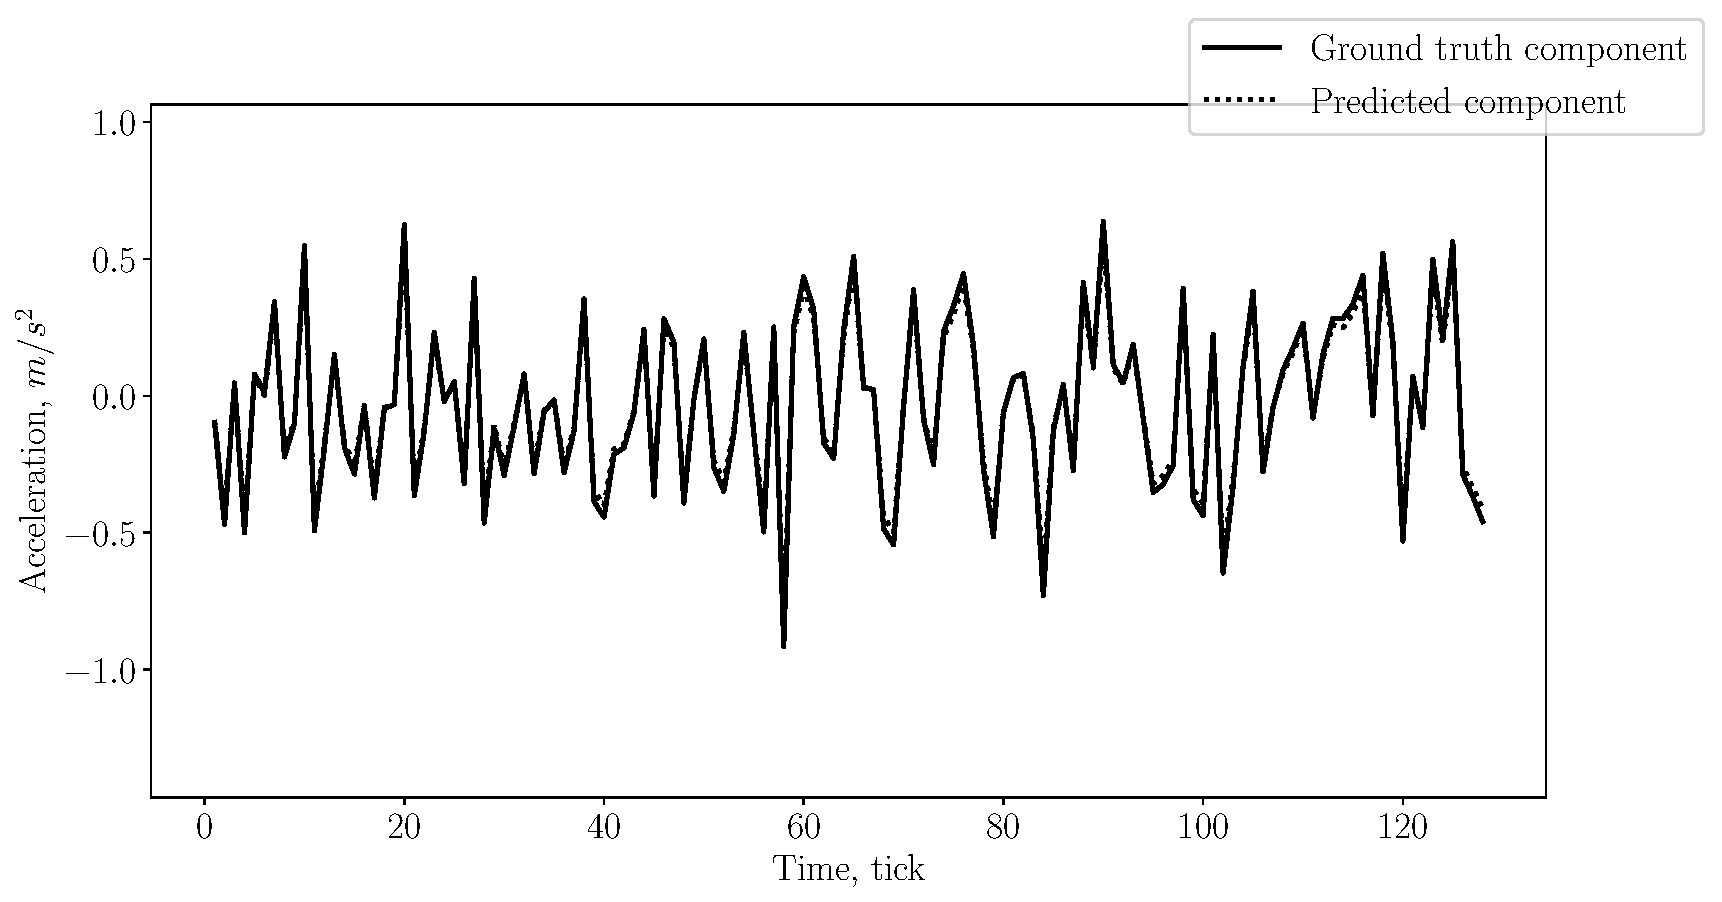
\includegraphics[scale = 0.42]{experiment4_1000.pickle_results_a.pdf}}\\
% \subfloat[]
 {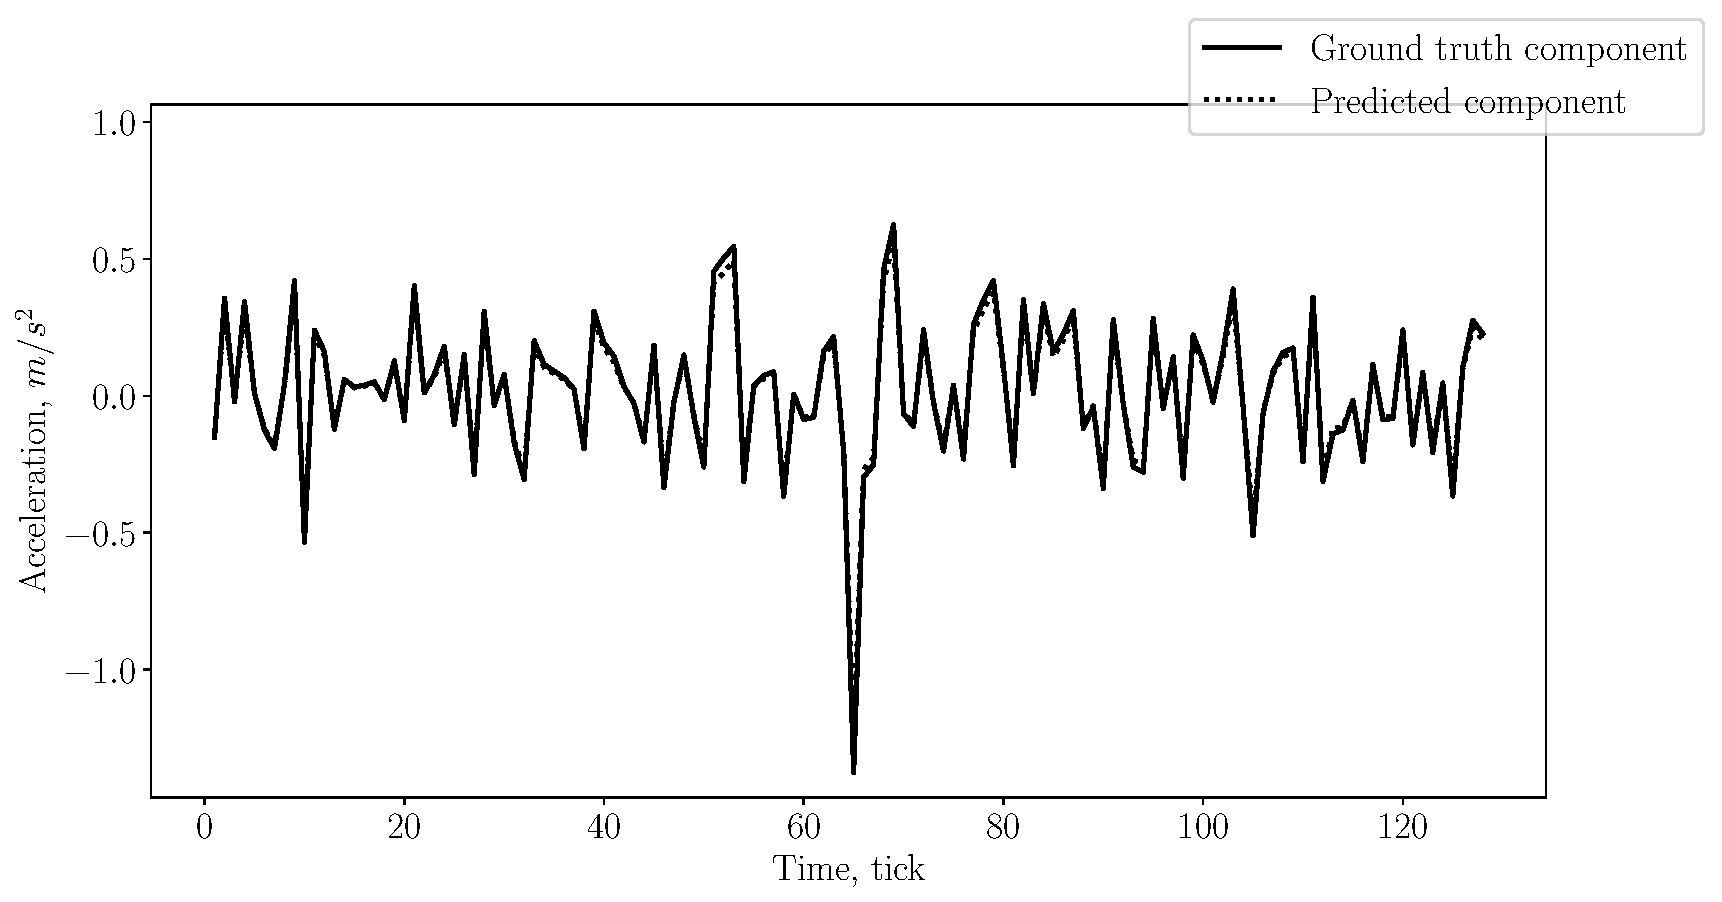
\includegraphics[scale = 0.42]{experiment4_1000.pickle_results_b.pdf}}}
 \caption{Time series of acceleration versus time for the test sample (a) first component, (b) second component}
 \label{fig: trajectory}
\end{figure}

\begin{figure}[!htbp]
\centering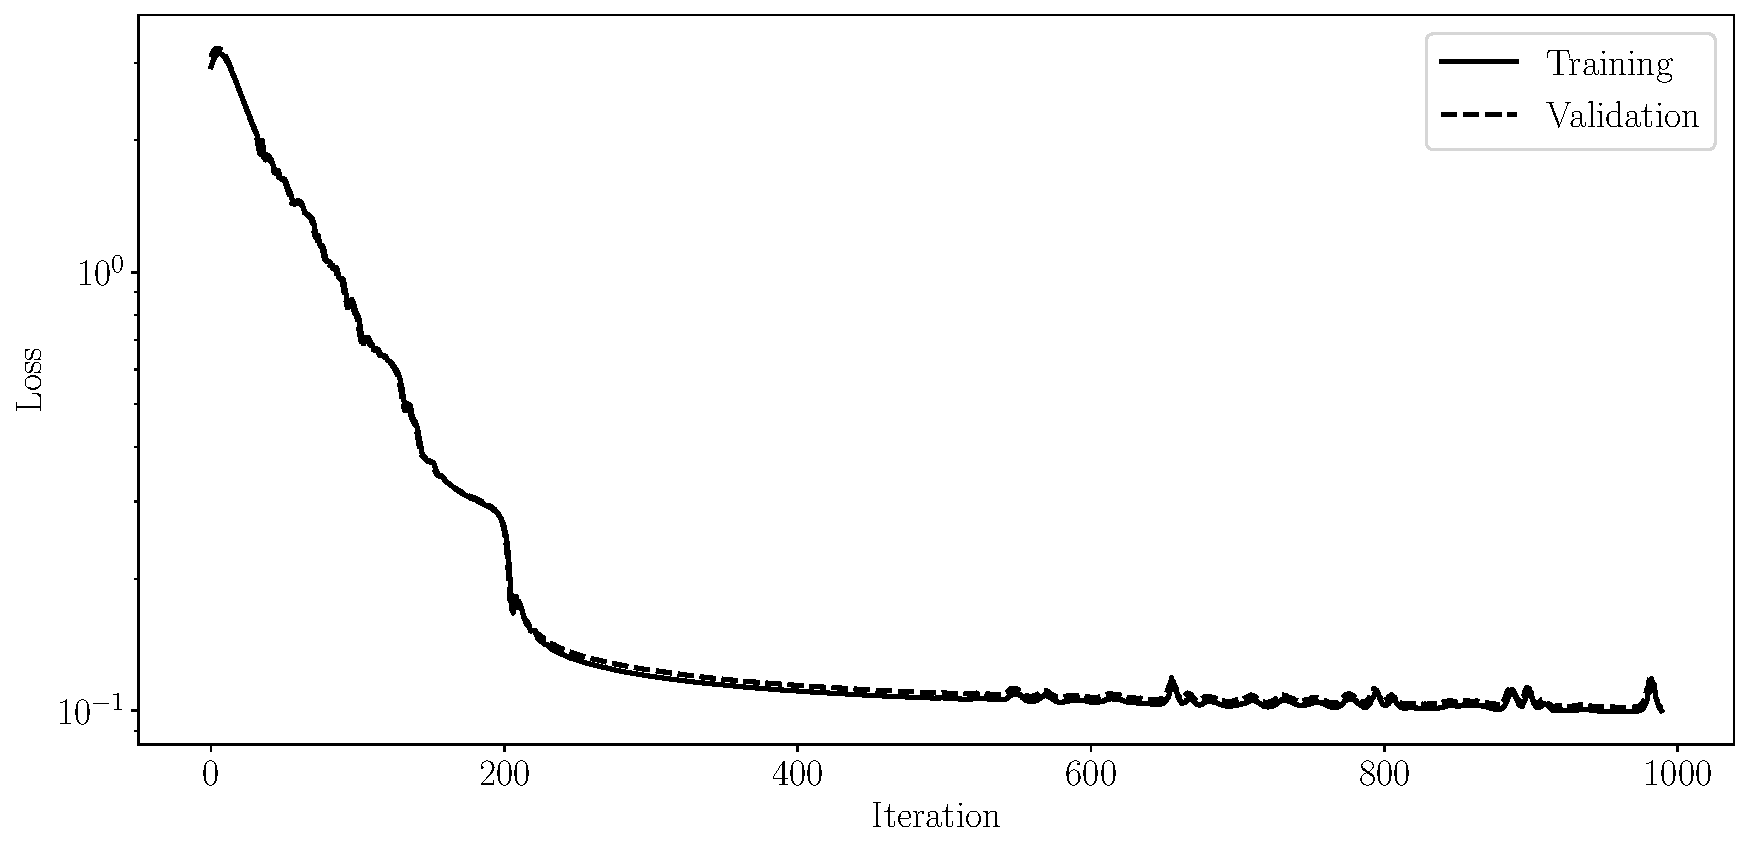
\includegraphics[scale = 0.42]{experiment4_1000.pickle_loss.pdf}
\caption{Model training graphics}
\label{fig: learning_rate}
\end{figure}

Figures \ref{fig: trajectory}, \ref{fig: learning_rate} show that the trajectories are exactly reconstructed by their Lagrangian, and we can predict them over a sufficiently large time interval, the losses on the test and training
samples are close, and the trajectories retain their appearance. This means that, according to the assumption, the Lagrangian space is a hidden space from which all trajectories are generated.

Thus~$\hat{L}_i$ vectorizes the~$X_i$ data for further classification. In the remark to lemma \ref{lemma2}, a norm
on the Lagrangian space is introduced, which represents it as a Hilbert space. Finally, the vectorization is taken from Remark \ref{remark3} in which the Lagrangian space is projected onto the Euclidean space $\mathbb{R}^n$. The vectorization of a trajectory corresponds to the vectorization of their
Lagrangians.

In contrast to \cite{article} , an additional regularization of the loss function is proposed.
Since in the regions where the eigenvalues of the Hessian
\[
\mathbf{H} = \left(\nabla_{\dot{\mathbf{q}}\dot{\mathbf{q}}} L\right)_{i j}=\frac{\partial^{2} L}{\partial \dot{q_{j}} \partial \dot{q}_{i}}
\]
tend to 0 the point of equilibrium is unstable, and the trajectories show nonphysical oscillations. Therefore, we introduce an additional term 
\[
\mathcal{L}_\text{restriction} =  \sum \alpha a(\beta(1 - \lambda(\mathbf{H})_i), 
\]
where~$a$ is some linear activation function, the best fit was %
$a = \text{SiLU} = x\sigma(x)$. The hyperparameters $\alpha, \beta$ are adjusted depending on the type of data, for this dataset~$\alpha = 5, \beta = 12$ are selected.

For the resulting Lagrangian estimator, we can sample the function values in any point $(\mathbf{q},\dot{\mathbf{q}})$. Accordingly, the norm on the basis of which the metric is constructed is sampled, and based on this metric, the underlying algorithms classify the trajectories.

Therefore, we first obtain a set of points at which the Lagrangian values are obtained. This
set is obtained before classification, and it is the same for all trajectories. Therefore, it is a
hyperparameter for the classifier. We obtain the set~$S = \{s_i\}$ of $N = 20000$ points $(\mathbf{q},\dot{\mathbf{q}})$ uniformly distributed on a cube~$-10 \le {x_i} \le 10$. Size
the cube is chosen so that it covers the points on which the Lagrangians are trained. The number of points for sampling should be chosen so that the estimate of the norm varies weakly
compared to its estimate.

For each object, the values~$X_i = \{AL(s_i)\}$ set of its features are obtained. The norm in this space corresponds to the usual Euclidean norm, and the basic algorithms of veto classification are used to classify objects in this space. We propose to classify objects by their features, i.e.,
sampled norm values.

To regularize the model and reduce dimensionality, we apply Principal Component Analysis and select the first three principal components in 2D and 3D plots in the Figures~\ref{fig:2D} and~\ref{fig:3D}. 
The data are separated into clusters. They visually fit the normal distribution so we use the Gaussian kernel in metric classifiers. The clusters are separated by linear surfaces in the presented Lagrangian space. 

\begin{figure}[!htbp]
\centering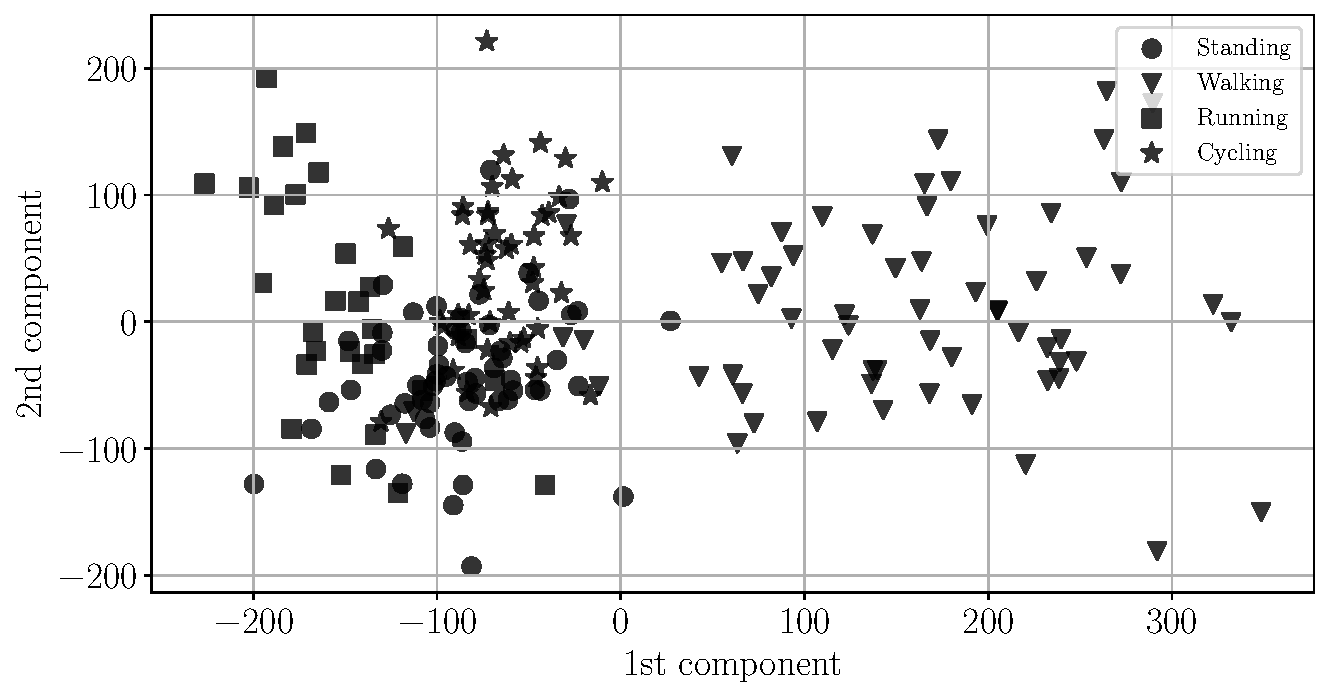
\includegraphics[scale = 0.5]{Data.pdf}
\caption{Projection of the Lagrangian estimates of $\hat{L}$ on a 2D-surface}
\label{fig:2D}
\end{figure}

\begin{figure}[!htbp]
\centering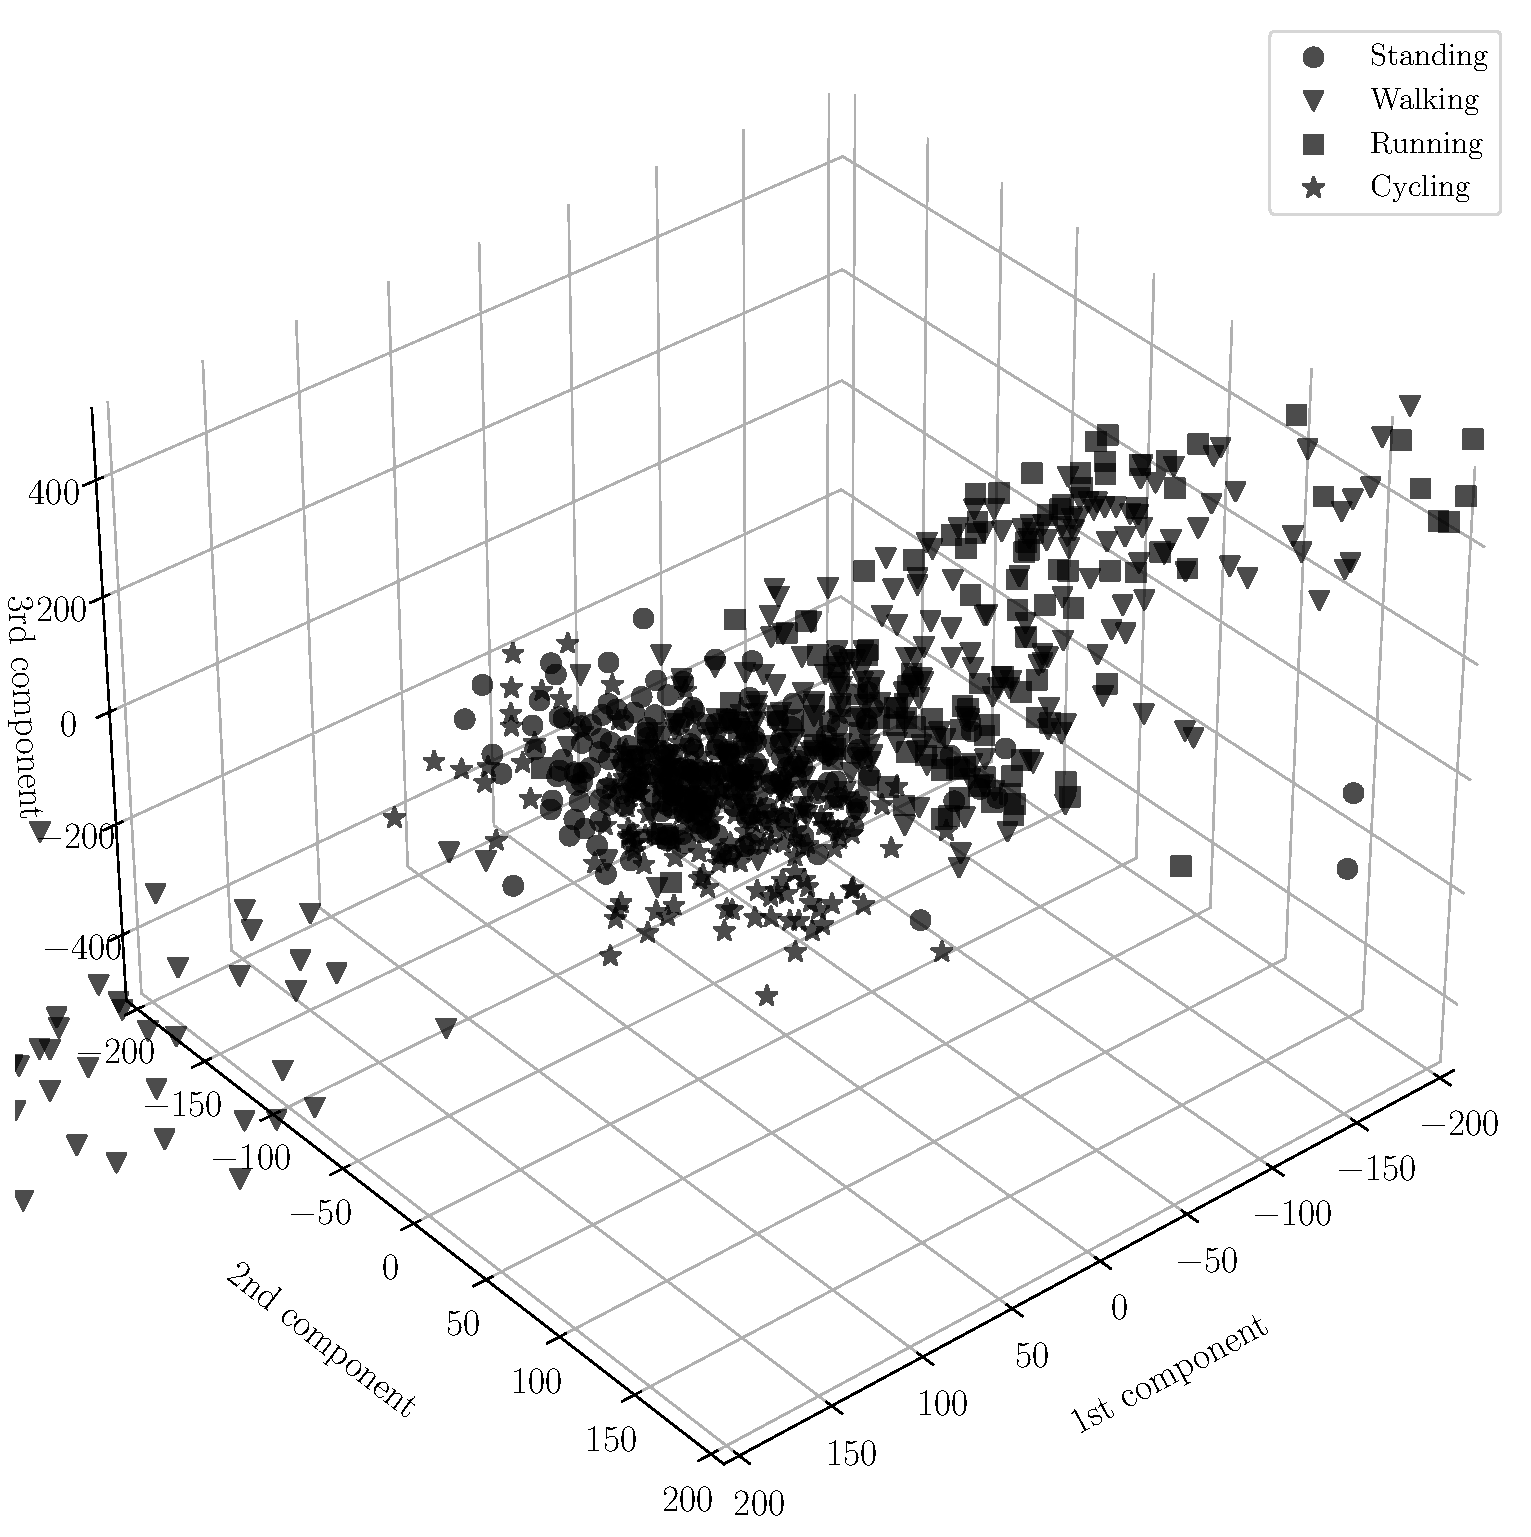
\includegraphics[scale = 0.4]{Data_3D.pdf}
\caption{Projection of the Lagrangian estimates of~$\hat{L}$ on a 3D-surface}
\label{fig:3D}
\end{figure}

The Random forest classifier was chosen for the study because it works well with any complex
datasets, linear regression and Gaussian process as simple enough classifiers that learn quickly
and therefore it is useful to know if they work on a dataset, and SVC with a Gaussian kernel
because visual analysis assumes that the data are normally distributed.

\begin{figure}[!htbp]
 \centering
 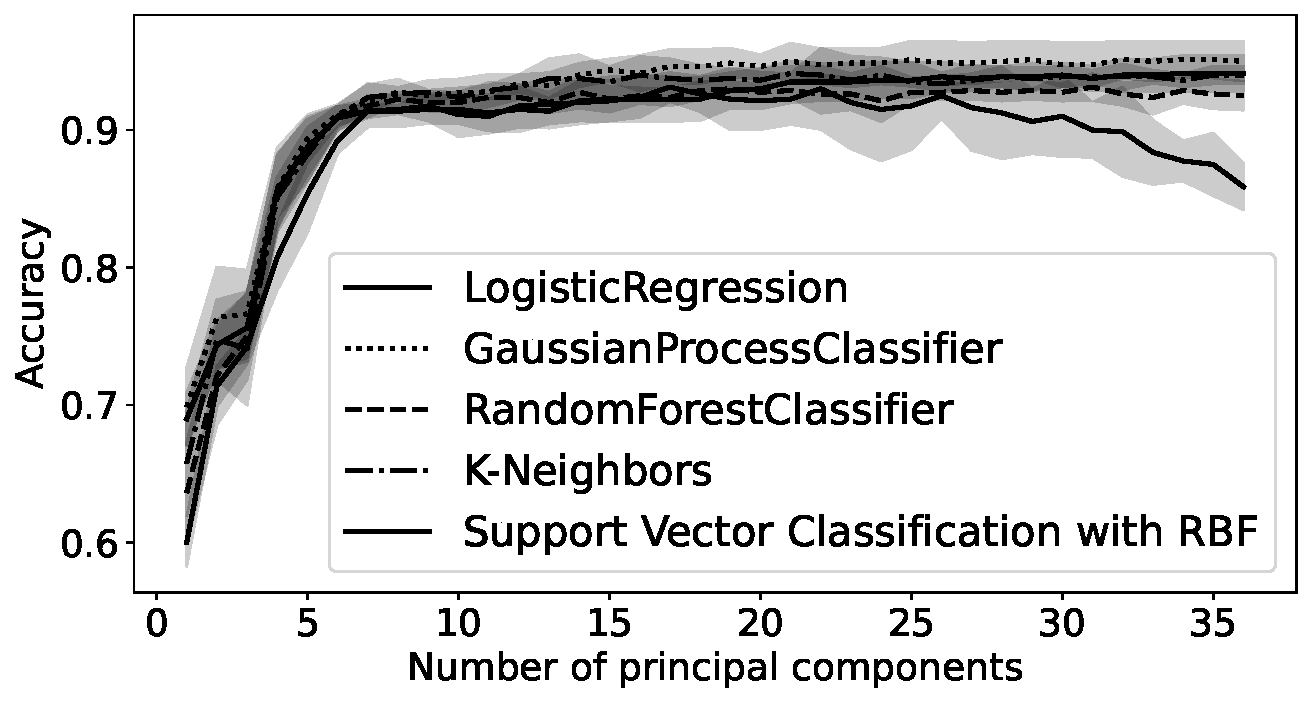
\includegraphics[scale = 0.5]{Accuracy.pdf}
 \caption{Classification accuracy of the selected methods depending on the number of principal
components}
 \label{fig: Accuracy}
\end{figure}

The Gaussian process classifier shows the best results according to all metrics in comparison to the rest of the models. The Metric classifiers, SVC and K-nearest neighbors, show similar results. Surprisingly, the logistic regression classifier recedes in accuracy, when the number of components is bigger than~$25$.  Among the the widely-used time series classification methods, the random forest classifier,  TimeSeriesForestClassifier from the Sktime library shows the accuracy $78\%$. It is much worse than the~LNN classifier. So, we select the Gaussian process classifier. 

\begin{table}[!htbp]
    \caption{Result of classifiers on the proposed data vectorization}
    \centering
    \begin{tabular}{|l|lll|}
    \hline
    \multicolumn{1}{|c|}{\multirow{2}{*}{Classifier}} & \multicolumn{3}{c|}{Metric}                                                                     	\\ \hhline{~---} 
    \multicolumn{1}{|c|}{}                               & \multicolumn{1}{l|}{Accuracy}         & \multicolumn{1}{l|}{Balanced-accuracy} & F1-macro        \\ \hline
    Logistic regression                              & \multicolumn{1}{l|}{$0.927 \pm  0.014$} & \multicolumn{1}{l|}{$0.924 \pm 0.13$}    & $0.927 \pm 0.14$  \\ \hline
    \textbf{Gaussian process}                                  & \multicolumn{1}{l|}{$\mathbf{0.946} \pm \mathbf{0.010}$}  & \multicolumn{1}{l|}{$\mathbf{0.941} \pm \mathbf{0.011}$}   & $\mathbf{0.946} \pm \mathbf{0.010}$ \\ \hline
    Random forest                                        & \multicolumn{1}{l|}{$0.932 \pm 0.007$}  & \multicolumn{1}{l|}{$0.928 \pm 0.008$}   & $0.933 \pm 0.008$ \\ \hline
    K-nearest neighbors                                  & \multicolumn{1}{l|}{$0.939 \pm 0.009$}  & \multicolumn{1}{l|}{$0.935 \pm 0.010$}   & $0.940 \pm 0.008$ \\ \hline
    SVC with Gaussian kernel                             & \multicolumn{1}{l|}{$0.933 \pm 0.012$}  & \multicolumn{1}{l|}{$0.927 \pm 0.01$3}   & $0.933 \pm 0.011$ \\ \hline
    \end{tabular}
    \label{table:classifictors}
\end{table}

\section{Conclusion}

The method provides a convenient way to project the data onto a plane for further visualization. Visual analysis of the plots shows that the represented Lagrangian space corresponds to the space of features that define a class of trajectories, i.e., they determine the type of motion. Similar results are shown by training linear models on the given vector space, the graphs show that linear models separate the classes represented in the dataset with an accuracy of 0.95. At the same time, the proposed vectorization is time-consuming and requires tuning the regularization parameters to achieve the necessary approximation accuracy on specific sets of trajectories.

Approximation of trajectories with dynamic system Lagrangians is a powerful tool for trajectory classification. It has many advantages over classification methods which do not use information about the physics of the system. This method is multivariate, there is no need to make  assumptions about the relationship between different components of trajectories. It is robust to changes in the data due to the proposed way of Lagrangian approximation. The proposed time series representation preserves assumptions about the physical nature of the signal measurements.
\textbf{}

\bibliography{lnn-bibliography}

\end{document}
